\subsection{Konceptualní, logická a fyzická úroveň pohledu na data}

TODO: sjednotit terminologii, snad to popisuje to co tu má být, ale zdroje jsou pochybné (Wikipedie tady neodvádí zrovna ideální práci a ČVUT Wiki se moc nerozepisuje).

\begin{definiceN}{Datové modelování}
\emph{Datové modelování} je proces vytvoření konkrétního datového modelu (schématu) databáze pomocí aplikace nějakého abstraktního databázového modelu. Datové modelování zahrnuje kromě definice struktury a organizace dat ještě další implictiní nebo explicitní omezení na data do struktury ukládaná. 
\end{definiceN}

\begin{obecne}{Vrstvy modelování}
Druhy datových modelů mohou být tří typů, podle tří různých pohledů na databáze (tři \uv{vrstvy}, které se navzájem doplňují):
\begin{pitemize}
    \item konceptuální schéma (datový model) -- nejabstraktnější, popisuje význam organizace databáze -- třídy entit a jejich vztahy.
    \item logické schéma -- popisuje význam konceptuálního schématu z hlediska databázové implementace -- popisy tabulek, programových tříd nebo XML tagů (podle zvoleného databázového modelu)
    \item fyzické schéma -- nejkonkrétnější, popisuje fyzické uložení dat a stroje na kterých systém poběží.
\end{pitemize}
Na tomto rozdělení je důležitá nezávislost jednotlivých vrstev -- takže se implementace jedné z nich může změnit, aniž by bylo nutné výrazně upravovat ostatní (samozřejmě musí zůstat konzistetní vzhledem k ostatním vrstvám). Během implementace nějaké databázové aplikace se začíná vytvořením konceptuálního schématu, pokračuje jeho upřesnění logickým schématem a naknec jeho fyzickou implementací podle fyzického schématu (modelu).
\end{obecne}

\begin{poznamka}
V tomto pohledu (který je podle standardu ANSI z r. 1975) jsou databázové modely, popsané v předchozí sekci, příklady abstraktních logických datových modelů. Někde je však tato úroveň označována jako \uv{fyzická} a \uv{jiná logická} se vtěsní ještě mezi ni a konceptuální.
\end{poznamka}


\begin{obecne}{Konceptuální schéma}
\emph{Konceptuální schéma} (datový model) popisuje podstatné objekty (\emph{třídy entit}, \uv{koncepty}), jejich charakteristiky (\emph{atributy}) a vztahy mezi nimi (asociace mezi dvojicemi tříd entit). Nepopisuje přímo implementaci v databázi, jen význam nějakého celku, který bude databází představován. Jde o modelování \uv{datové reality}, z pohledu uživatele (analytika, konstruktéra databáze).

\medskip
\begin{priklady}
Pár příkladů vztahů mezi třídami entit (z Wikipedie):
\begin{pitemize}
    \item Each PERSON may be the vendor in one or more ORDERS.
    \item Each ORDER must be from one and only one PERSON.
    \item PERSON is a sub-type of PARTY. (Meaning that every instance of PERSON is also an instance of PARTY.)
\end{pitemize}
\end{priklady}
De-facto standardem pro konceptuální datové modelování jsou \emph{ER-diagramy} (entity-relationship diagramy). Hodí se hlavně pro \uv{plochá} formátovaná data (takže třeba pro objektové nebo relační databáze, ale ne pro XML apod.). Používají dva typy \uv{objektů} -- \emph{entity} (třídy entit) a \emph{vztahy}. Jde o obdobu UML z objektového programování. Příklad ER-diagramu se vztahem dvou entit je na následujícím obrázku (popisuje i další vlastnosti -- atributy entit a kardinality vztahů):
\begin{center}
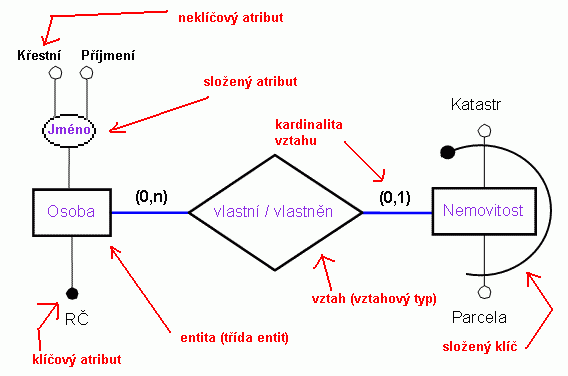
\includegraphics[width=14cm]{informatika/databazy/obrazky/er-schema.png}

(Obrázek je upravený, rozšířený a popsaný příklad ze slidů Dr. T. Skopala k Databázovým systémům)
\end{center}
\end{obecne}

\begin{obecne}{Logické schéma}
\emph{Logické schéma} je datový model organizace nějakého specifického celku pomocí jednoho z databázových modelů -- podle databázových modelů popsaných v předchozí sekci, tj. např. pomocí relačních tabulek, objektových tříd nebo XML. Svojí úrovní abstrakce se nachází mezi konceptuálním a fyzickým schématem.
\end{obecne}

\begin{obecne}{Fyzické schéma}
\emph{Fyzické datové modely} jsou modely, ktere používají databazové stroje směrem k nižším vrstvám (operačního) systému. V zásadě jde o různé způsoby fyzického uložení dat (tedy schémata organizace souborů) -- sekvenční soubory, B-stromy apod.
\end{obecne}

